
\documentclass[fleqn,addpoints]{exam}
\usepackage{amsmath}
\usepackage{graphicx}
\usepackage{booktabs}
\usepackage{float}
\usepackage{caption}
\usepackage{polynom}
\usepackage{mdwlist}
\usepackage{cancel}

\usepackage{unitsdef} 
\newunit{\inch}{in}
\newunit{\mile}{mile}
\newunit{\mph}{mph}
\newunit{\foot}{ft}
\newunit{\knot}{knot}
\newunit{\gallon}{gallon}

\bracketedpoints
\everymath{\displaystyle}

\printanswers

% \begin{figure}[H]
%   \centering
%   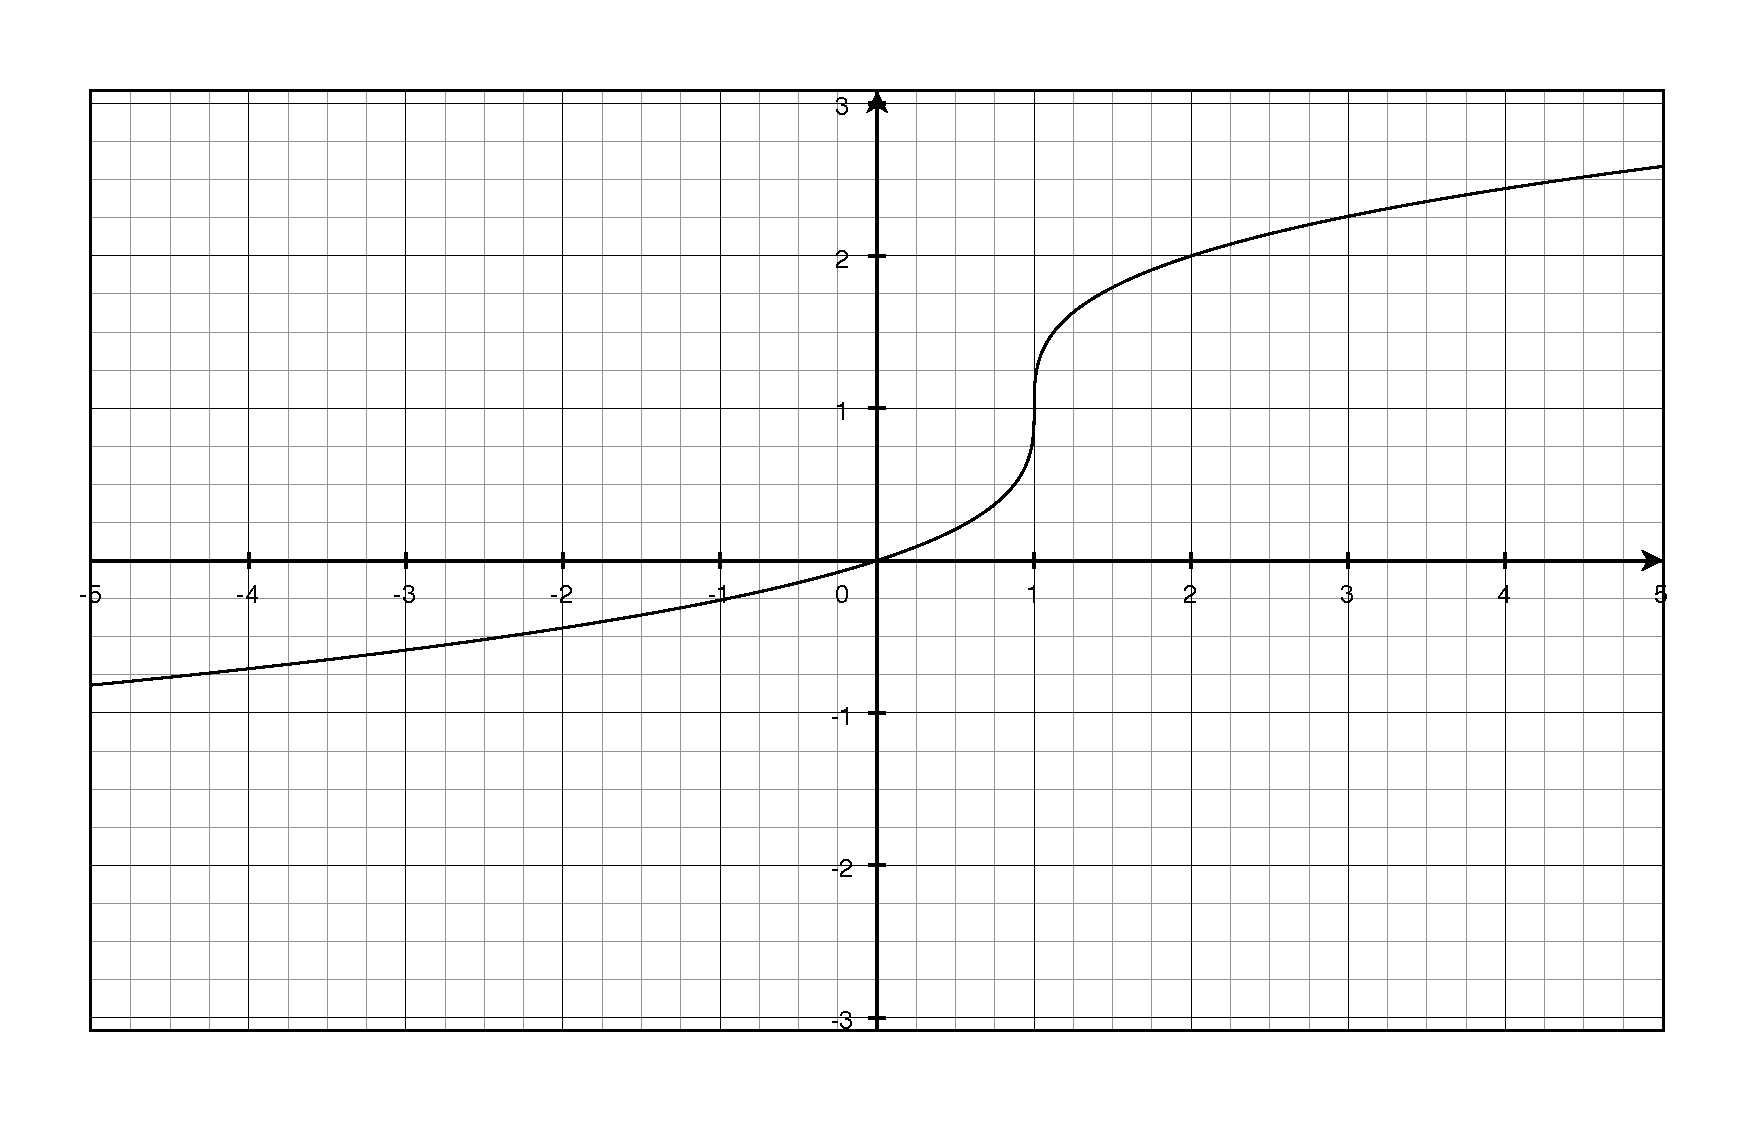
\includegraphics[scale=.3]{question7.eps}
%   \caption*{Question 7}
% \end{figure}

% \begin{tabular}{cc}
% \toprule
% period & amplitude \\
% \midrule
%   $\pi$ & $2$ \\
% \bottomrule
% \end{tabular}


\ifprintanswers
\usepackage{2in1, lscape}
\fi

\title{Math 263A Sample Final Four}

\date{October 25, 2012}

\author{}

\begin{document}

% from winter 2009 final

\maketitle  

\begin{questions}

\question
Sketch the graph of a function $f$ for which $f(0) = 0$, $f'(0) = 2$, $f'(1) = 0$, and $f'(2) = 2$.

\begin{solution}
I can't get my computer to draw this graph.
\end{solution}

%% \question
%% Prove that:
%% \[
%%   \lim_{x \to 0^+} \sqrt{x} \left[1 + \sin^2 \left(\frac{1}{x} \right) \right] = 0
%% \]

\question Find the limit:
\[
  \lim_{x \to \infty} \frac{x^3 + 5x}{3x^3 - x^2 + 4}
\]

\begin{solution}
\begin{align*}
  \lim_{x \to \infty} \frac{x^3 + 5x}{3x^3 - x^2 + 4} &=   \lim_{x \to \infty} \frac{1 + 5/x^2}{3 - 1/x + 4/x^3} \\
  &= \frac{1}{3} \\
\end{align*}
\end{solution}

\question Verify that the function satisfies the hypotheses of the {\em Mean Value Theorem}.  Then find all numbers $c$
that satisfy the conclusion of the {\em Mean Value Theorem}.
\[
  f(x) = x^3 + x - 1 \text{, } [0, 1]
\]

\begin{solution}
Since $f$ is a polynomial, it is continuous and differentiable everywhere.

The mean value for the interval is:
\[
  f_{mean} = \frac{f(1) - f(0)}{1} = \frac{1 - (-1)}{1} = 2
\]

find the derivative:
\[
  f'(x) = 3x^2 + 1
\]

find the points where the derivative is 2:
\begin{align*}
  3x^2 + 1 &= 2 \\
  3x^2 &= 3 \\
  x &= \pm 1
\end{align*}

Only $x = 1$ is in the target interval.

\end{solution}

\question
Show that the equation $x^5 + 10x + 3 = 0$ has exactly one real root.
\begin{solution}

We can use the {\em Intermediate Value Theorem} to show that $f$ has at least one root by showing that there are some
values where $f(x) < 0$ and other values where $f(x) > 0$.  For example, $f(-1) < 0$ and $f(1) > 0$.  Therefore, $f$ has
at least one real root in the interval $(-1, 1)$.

We can use the derivative to show that $f$ doesn't have more than one real root.  The derivative is:
\[
  f'(x) = 5x^4 + 10
\]
Notice that $f'(x) > 0$ for all $x$, so $f$ is constantly increasing.  Since $f$ is constantly increasing it can only
cross the x-axis once.

\end{solution}

\ifprintanswers
\pagebreak
\fi

\question Find the derivative of the function at $r = 2$: $y = \frac{r^2}{1 + \sqrt{r}}$
\begin{solution}
\begin{align*}
  y &= \frac{r^2}{1 + r^{1/2}} \\
  y' &= \frac{(1 + r^{1/2}) \cdot 2r - r^2 \left(\cfrac{1}{2} r^{-1/2} \right) } {(1 + r^{1/2})^2} \\
     &= \frac{4r + 3r^{3/2}}{2 (1 + r^{1/2})^2} \\
\end{align*}

If you plug in $r = 2$ and to a bunch of simplification, you'll find that $y'(2) = \sqrt{2}$.  On the test, however, you
can just plug it in to your calculator.

\end{solution}


%% \question A man starts walking north at $4 \foot / \second$ from a point $P$. Five minutes later a woman starts walking
%% south at $5 \foot / \second$ from a point $500 \foot$ due east of point P. At what rate are the people moving apart 
%% $15 \minute$ after the woman starts walking.

\question A farmer has $1200 \foot$ of fencing and wants to fence off a rectangular field that borders a straight
river. He needs no fence along the river. What are the dimensions of the field that has the largest area?

\begin{solution}
If $x$ and $y$ are the lengths of the two sides, with $y$ the side opposite the river:
\begin{align*}
  A &= xy \\
  P &= 2x + y \\
\end{align*}

Since we want to maximize area, we need to solve the perimeter equation for $y$ and substitute the result in the area
equation:
\begin{align*}
  y &= P - 2x \\
  A &= x(P - 2x) \\
    &= Px - 2x^2 \\
\end{align*}

differentiate the area equation:
\begin{align*}
  A &= Px - 2x^2 \\
  A' &= P - 4x \\
\end{align*}

set the result equal to zero:
\begin{align*}
  P - 4x &= 0 \\
  x &= \frac{P}{4} \\
\end{align*}

For our problem, $P = 1,200$:
\begin{align*}
  x &= 300 \\
  y &= 600 \\
\end{align*}

The maximum area is: $A = 300 \cdot 600 = 180,000 \foot^2$

\end{solution}

\question
Find the point on the parabola $x + y^2 = 0$ that is closest to the point $(0, -3)$.

\begin{solution}
I got this problem from another text book.  It didn't come from an OU sample final.  It looks straightforward, but
solving the final equation requires remembering a technique from pre-calculus.  Anyway, here's how I did it.

the distance squared is:
\[
  r^2 = x^2 + (y + 3)^2
\]

Since $x = -y^2$, we can get rid of $y$ in the distance equation:
\[
  r^2 = y^4 + (y + 3)^2
\]

Minimizing distance squared gives the same result as minimizing distance, and the differentiation is easier:
\[
  D_x (y^4 + (y + 3)^2) = 4y^3 + 2y + 6
\] 

To find the minimum, set this equal to zero and solve for $y$.  This is a bit tricky, since the equation is a 3rd degree
equation.
\begin{align*}
  4y^3 + 2y + 6 &= 0 \\
  2y^3 + y + 3 &= 0 \\
\end{align*}

If you remember the {\em Rational Zero Test} from precalculus, you can find that the candidate solutions are: 
$\left\{\pm 1, \pm 3, \pm \frac{2}{3} \right\}$. When you try these, you find that $y = -1$ works, so the 
closest point is $(-1, -1)$

I'm pretty sure there won't be a problem that requires this technique on the final---sorry about including it on the practice final.

\end{solution}

%% \question Find the limit. 
%% \[
%%   \lim_{x \to \frac{\pi}{2}^+} \frac{\cos x}{1 - \sin x} 
%% \]

\question
Find the absolute maximum and minimum values of $f$ on the given interval. 
\[
  f(x) = x^3 - 6x^2 + 9x + 2 \text{, } [-1, 4].
\]

\begin{solution}
differentiate:
\[
  f'(x) = 3x^2 - 12x + 9
\]

set equal to zero and solve:
\begin{align*}
  3x^2 - 12x + 9 &= 0 \\
  x^2 - 4x + 3 &= 0 \\
  (x - 3)(x - 1) &= 0 \\
  x &= \{1, 3\}
\end{align*}

try all the candidate values, including the endpoints to see which ones are maximum and minimum:

\begin{tabular}{lrrrr}
\toprule
$x$  & $-1$    & 1 & 3 & 4 \\
\midrule
$f(x)$ & $-14$ & 6 & 2 & 6 \\
\bottomrule
\end{tabular}

So the the minimum is $(-1, 14)$ and the maximums are $(1, 6)$ and $(4, 6)$.

\end{solution}

\question
differentiate:
\[
  y = A + \frac{B}{x} + \frac{C}{x^2}
\]

\begin{solution}
\begin{align*}
  y &= A + Bx^{-1} + Cx^{-2} \\
  y' &= A - Bx^{-2} - 2Cx^{-3} \\
     &= A - \frac{B}{x^2} - \frac{2C}{x^3} \\
\end{align*}

\end{solution}

\question
If $y = x^3 + 2x$ and $\frac{dx}{dt} = 5$, find $\frac{dy}{dt}$ when $x = 2$.

\begin{solution}
\begin{align*}
  y &= x^3 + 2x \\
  \frac{dy}{dt} &= (3x^2 + 2) \cdot \frac{dx}{dt} \\
  &= (3 \cdot 4 + 2) \cdot 5 \\
  &= 70 \\
\end{align*}

\end{solution}

\ifprintanswers
\pagebreak
\fi

\question
Find $\frac{dy}{dx}$:
\[
  y = \frac{\sqrt{x} - 1}{\sqrt{x} + 1}
\]

\begin{solution}
\begin{align*}
  y' &= \frac{(x^{1/2} + 1) \cdot \frac{1}{2} x^{-1/2} - (x^{1/2} - 1) \cdot \frac{1}{2} x^{-1/2}}{(x^{1/2} + 1)^2} \\
  &= \frac{1}{\sqrt{x}(\sqrt{x} + 1)^2}
\end{align*}
  
\end{solution}

\question
If a ball is thrown vertically upward with a velocity of $80 \foot / \second$, then its height after $t \second$ is:
$s = 80t - 16t^2$.
\begin{parts}
\part What is the maximum height reached by the ball?
\begin{solution}
The maximum height is when the velocity is zero when the ball reaches the top and turns around.
\begin{align*}
  v &= 80 - 32t \\
  80 - 32t &= 0 \\
  t &= 2.5 \second \\
\end{align*}

The height when $t = 2.5 \second$ is: $s = 100 \foot$
\end{solution}

\part What is the velocity of the ball when it is $96 \foot$ from the ground on its way up?
\begin{solution}
Find the time when the ball is $96 \foot$ from the ground:
\begin{align*}
  80t - 16t^2 &= 96 \\
  16t^2 - 80t + 96 &= 0 \\
  t^2 - 5t + 6 &= 0 \\
  (t - 3)(t - 2) \\
  t &= \{2, 3\} \second \\
\end{align*}
Since the peak is at $2.5 \second$, the point on the way up is $t = 2 \second$.

The velocity at this time is: 
\[
  v(2) = 80 - 32 \cdot 2 = 1.25 \foot/\second
\]

\end{solution}

\end{parts}

\question
Two cars start moving from the same point.  One travels south at 60 mph and the other travels west at 25 mph.  At what
rate is the distance between the cars changing two hours later?

\begin{solution}
The rate the distance between the cars is changing is:
\begin{align*}
  r^2 &= x^2 + y^2 \\
  \frac{dr}{dt} &= \frac{x}{r} \frac{dx}{dt} + \frac{y}{r} \frac{dy}{dt} \\
\end{align*}

The facts from the problem are:
\begin{itemize}
  \item $\frac{dx}{dt} = -25$
  \item $\frac{dy}{dt} = -60$
  \item $x = -50$ 
  \item $y = -120$ 
  \item $r = 130$
\end{itemize}

plug these numbers into the rate equation:
\begin{align*}
  \frac{dr}{dt} &= \frac{x}{r} \frac{dx}{dt} + \frac{y}{r} \frac{dy}{dt} \\
    &= \frac{50}{130} \cdot 25 + \frac{120}{130} \cdot 60 \\
    &= 65 \mph \\
\end{align*}

\end{solution}

\question
\begin{parts}
  \part Find the derivative of the function.
\begin{solution}
\begin{align*}
    f(x) &= x (x + 3)^{1/2} \\
    f'(x) &= x \cdot \frac{1}{2} (x + 3)^{-1/2} + (x + 3)^{1/2} \\
          &= \frac{3x + 6}{\sqrt{x + 3}} \\
\end{align*}
\end{solution}

  \part Find the vertical and horizontal asymptotes.
\begin{solution}
There aren't any asymptotes.
\end{solution}

  \part Find the intervals on which $f$ is increasing or decreasing. 
\begin{solution}
\begin{align*}
  3x + 6 &= 0 \\
  x &= -2 \\
\end{align*}
\begin{itemize*}
\item decreasing: $(-3, -2)$
\item increasing: $(-2, \infty)$
\end{itemize*}
\end{solution}
  \part Find the intervals of concavity and the inflection points.
\begin{solution}
\begin{align*}
  f''(x) &= \frac{(x + 3)^{1/2} \cdot 3 - (3x + 6)(x + 3)^{-1/2}}{x + 3} \\
         &= \frac{3x + 12}{4(x + 3)^{3/2}}  
\end{align*}
Since $f''$ is always positive, $f$ is always concave up and there aren't any inflection points.
\end{solution}

  \part Find the local maximum and minimum values of $f$.
\begin{solution}
  From part (c), is a local minimum at $(-2, -2)$.
\end{solution}

  \part Use the information from (a)-(e) to sketch the graph.
\begin{solution}
\begin{figure}[H]
  \centering
  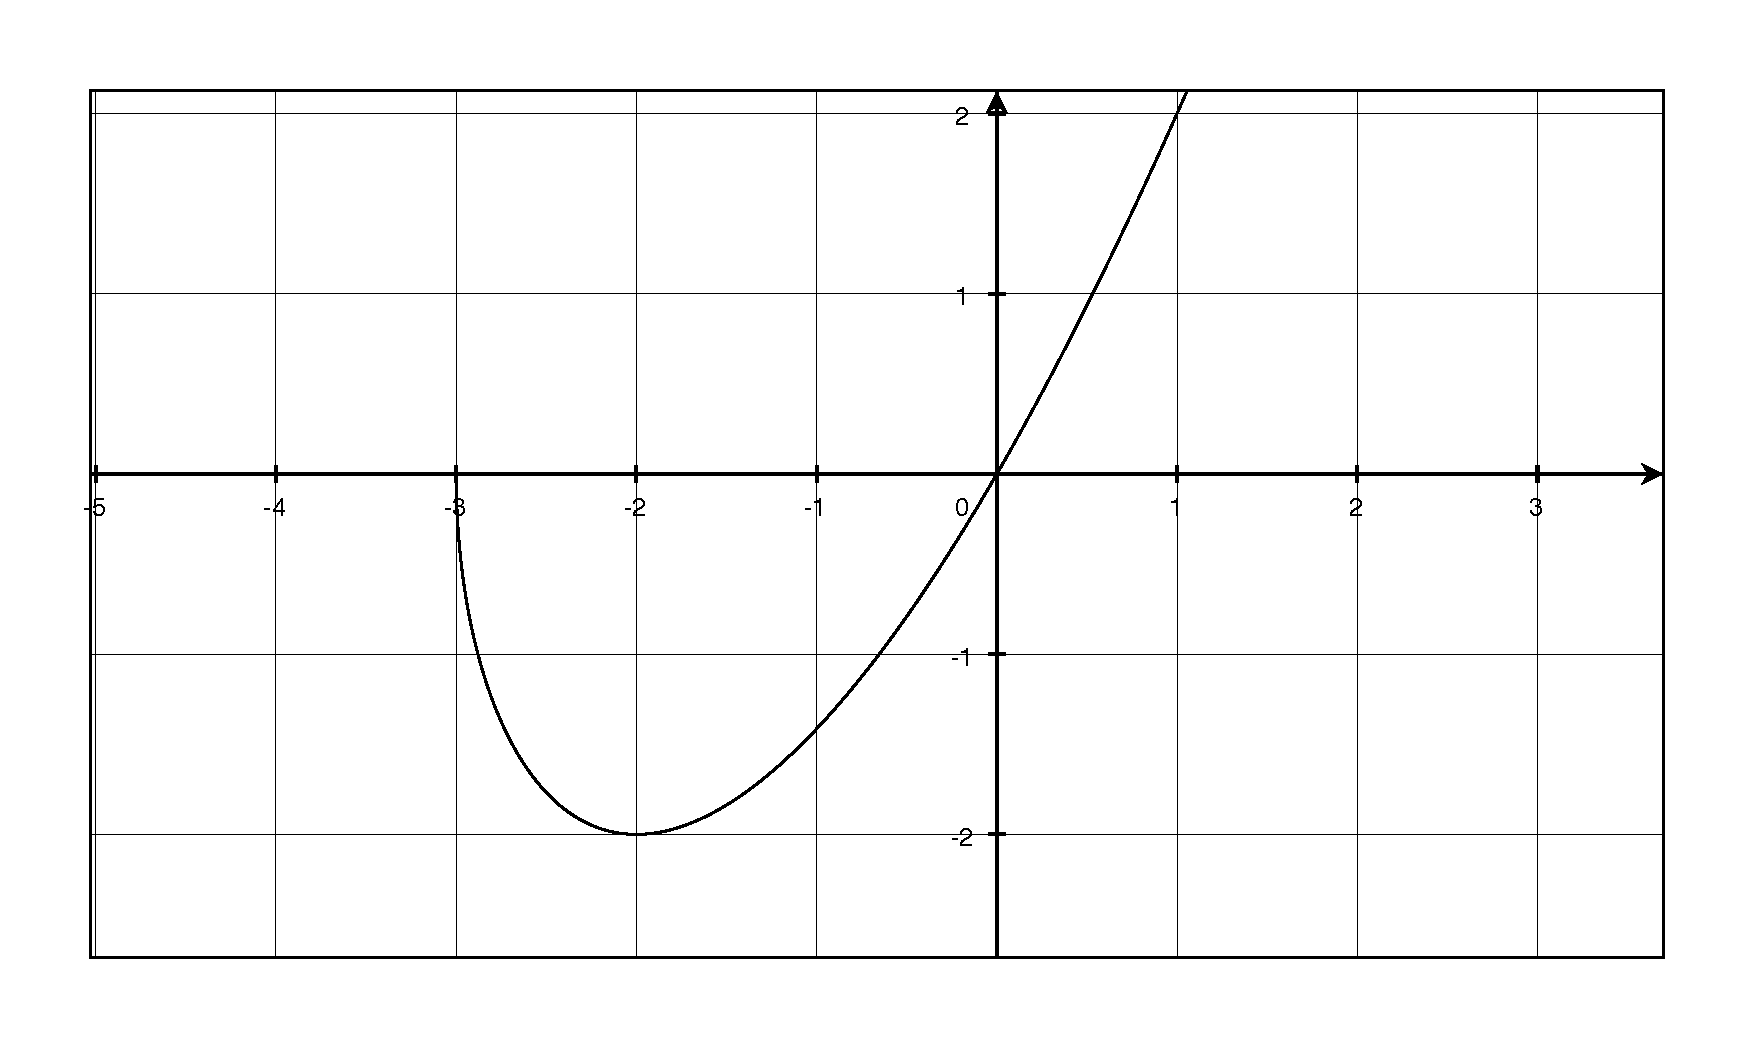
\includegraphics[scale=.3]{final_4_q14.eps}
  \caption*{Question 14}
\end{figure}
\end{solution}


\end{parts}
\[
  f(x) = x \sqrt{x+3}
\]

\ifprintanswers
\pagebreak
\fi

\question
\begin{parts}
  \part Find the derivative of the function.
\begin{solution}
\begin{align*}
  f'(x) &= \frac{(x + 1) \cdot 2 - 2x}{(x + 1)^2} \\
        &= \frac{2}{(x + 1)^2} \\
\end{align*}

\end{solution}

  \part Find the vertical and horizontal asymptotes.
\begin{solution}
horizontal asymptote:
\[
  \lim_{x \to \infty} \frac{2x}{x + 1} = \lim_{x \to \infty} \frac{2}{1 + 1/x} = 2 
\]
There is a horizontal asymptote at $y = 2$.

Since the numerator is non-zero and the denominator is zero when $x = -1$, there is a vertical asymptote at $x = -1$.
\end{solution}

  \part Find the intervals on which $f$ is increasing or decreasing. 
\begin{solution}
$f'$ is always positive, so $f$ is always increasing, except for $x = -1$ where it is not defined.
\end{solution}

  \part Find the intervals of concavity and the inflection points.
\begin{solution}
\begin{align*}
  f''(x) &= \frac{-4}{(x + 1)^3}
\end{align*}

The only inflection point is when $f''(x)$ is undefined at $x = -1$.
\begin{itemize*}
  \item concave up: $(-\infty, -1)$
  \item concave down: $(-1, \infty)$
\end{itemize*}

\end{solution}

\ifprintanswers
\pagebreak
\fi

  \part Find the local maximum and minimum values of $f$.
\begin{solution}
  Since $f'$ is always positive, there aren't any local maximum or minimum values.
\end{solution}

  \part Use the information from (a)-(e) to sketch the graph.
\begin{solution}
\begin{figure}[H]
  \centering
  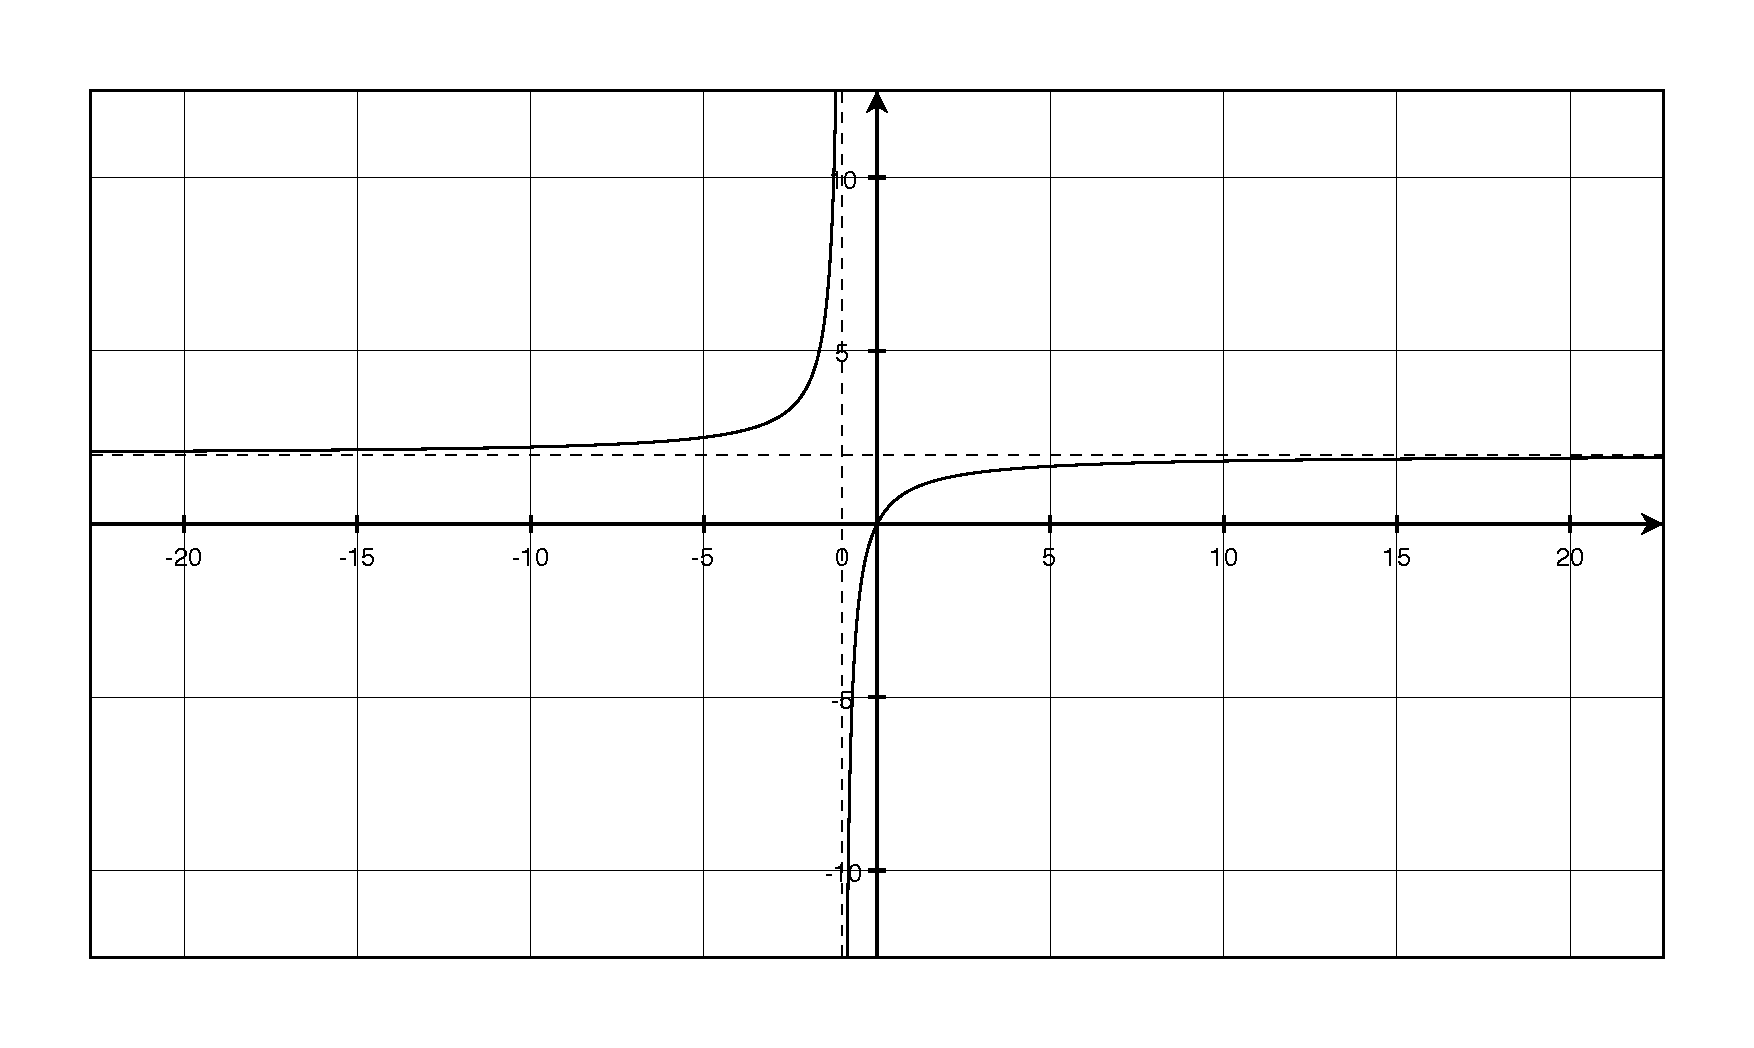
\includegraphics[scale=.3]{final_4_q15.eps}
  \caption*{Question 15}
\end{figure}
\end{solution}

\end{parts}
\[
  f(x) = \frac{2x}{x + 1}
\]

\end{questions}

\end{document}
